\chapter{Multi-Paradigm Programming con JavaScript}

\section{Il lato funzionale}

Le \textbf{funzioni} sono introdotte dalla keyword \texttt{function}:
\begin{itemize}
    \item il nome è \textit{opzionale}, possibili funzioni anonime
    \item sintassi alternativa: \textit{lambda expression}
    \item \textit{function expression} vs \textit{function declaration}
    \item non si usa la keyword \texttt{void}
\end{itemize}

Parametri privi di dichiarazione di tipo
\begin{minted}[bgcolor=lightgray,framesep=2mm,baselinestretch=1.2,fontsize=\footnotesize,escapeinside=||,mathescape=true]{js}
// funzione
function sum(a, b) { return a + b }
// procedura no return
function printSum(a, b) {
    document.write(a + b)
}
// funzione anonima
var sum = (a, b) => a + b
\end{minted}

A differenza di molti altri linguaggi, i parametri \textit{attuali} possono non corrispondere in numero ai parametri \textit{formali}:
\begin{itemize}
    \item se sono più, extra ignorati
    \item se sono meno, mancanti \texttt{undefined}
\end{itemize}

\subsection{Funzioni come first class entities}
In javascript, una funzione è una entità-oggetto, manipolabile come ogni altro tipo:
\begin{itemize}
    \item assegnabile a variabili
    \begin{itemize}
        \item[] \texttt{var f = function(x) \{ return x / 10 \}}
        \item[] \texttt{var f = x => x / 10}
    \end{itemize}
    \item definita e usata al "volo" con un \textit{function literal}
    \begin{itemize}
        \item[] \texttt{var z = function(y) \{ return y + 1 \}(8)}
        \item[] \texttt{var z = (y = > y + 1)(8)}
    \end{itemize}
    \item passata come argomento
    \begin{itemize}
        \item[] \texttt{var p = ff(f)}
    \end{itemize}
    \item restituita da funzione factory
    \begin{itemize}
        \item[] \texttt{var f = fgen(...)}
    \end{itemize}
\end{itemize}

\subsection{Function expression vs function declaration}
La \textbf{function expression} assegna una funzione a una variabile
\begin{itemize}
    \item il nome della funzione non è essenziale
    \item lo scope del nome, se presente, è il \textit{corpo della funzione} (utile in chiamate ricorsive)
\end{itemize}
\begin{minted}[bgcolor=lightgray,framesep=2mm,baselinestretch=1.2,fontsize=\footnotesize,escapeinside=||,mathescape=true]{js}
var f = function g(x) { return x / 10 }
g(32) //errore, nome g non definito
\end{minted}

La \textbf{function declaration} introduce una funzione senza assegnarla a una variabile
\begin{itemize}
    \item il nome è essenziale
    \item lo scope è l'\textit{ambiente di definizione} della funzione
\end{itemize}
\begin{minted}[bgcolor=lightgray,framesep=2mm,baselinestretch=1.2,fontsize=\footnotesize,escapeinside=||,mathescape=true]{js}
function g(x) { return  x / 10 }
g(32) //nome g definito
\end{minted}

\subsection{Funzioni innestate e chiusure}
Si possono definire funzioni dentro altre, nasce quindi la discussione delle \textbf{chiusure}, javascript segue la chiusura \textit{lessicale}.

Una chiusura nasce quando una funzione innestata fa riferimento a \textit{variabili della funzione esterna}.

\subsection{Currying}
Un caso interessante di chiusura è la possibilità di simulare una funzione a N argomenti con N funzioni a 1 argomento.

Si può esprimere una funzione come questa
\begin{minted}[bgcolor=lightgray,framesep=2mm,baselinestretch=1.2,fontsize=\footnotesize,escapeinside=||,mathescape=true]{js}
function sum(a, b) { return a + b }
var result = sum(3, 4)
\end{minted}
in una forma diversa, basata su una funzione "esterna" con argomento \texttt{a}, che restituisce una funzione "interna" con argomento \texttt{b}.
\begin{minted}[bgcolor=lightgray,framesep=2mm,baselinestretch=1.2,fontsize=\footnotesize,escapeinside=||,mathescape=true]{js}
function sum(a) { return function(b) { return a + b } }
var result = sum(3)(4)
\end{minted}

Questa possibilità si chiama \textbf{currying}.

É possibile utilizzare anche la definizione tramite lambda con la seguente sintassi
\begin{minted}[bgcolor=lightgray,framesep=2mm,baselinestretch=1.2,fontsize=\footnotesize,escapeinside=||,mathescape=true]{js}
sum = a => b => a + b
var result = sum(3)(4)
\end{minted}
Il currying è concettualmente interessante perché indica che l'unico "ingrediente" fondamentale per esprimere qualunque funzione sono le \textit{funzioni a un argomento}.

\subsection{Utilizzi chiusure}

\subsubsection{Rappresentare uno stato privato e nascosto}
Si può ottenere una \textit{proprietà privata} tramite una chiusura, mappando lo stato su un argomento della funzione "generatrice"
\begin{minted}[bgcolor=lightgray,framesep=2mm,baselinestretch=1.2,fontsize=\footnotesize,escapeinside=||,mathescape=true]{js}
function incBy2From(x) {
    return function() { return x += 2 }
}
\end{minted}

Da ogni invocazione di \texttt{incBy2From}, nasce un nuova funzione, che ha uno "stato" interno privato e utilizza come punto di partenza il parametro passato al generatore.

Altro esempio, generatore di contatori
\begin{minted}[bgcolor=lightgray,framesep=2mm,baselinestretch=1.2,fontsize=\footnotesize,escapeinside=||,mathescape=true]{js}
function genContatore(){
    var contati=0;
    function tick() { return contati++; }
    function num() { return contati;}
    //metodo per restituire più funzioni di accesso
    return { num, tick };
}
\end{minted}

\subsubsection{Realizzare un canale di comunicazione privato}
Si può ottenere un canale di comunicazione privato, mettendo in una chiusura sia lo \textbf{stato} che i due \textbf{metodi accessor}.

Si utilizza un array di due funzioni per restituirli
\begin{minted}[bgcolor=lightgray,framesep=2mm,baselinestretch=1.2,fontsize=\footnotesize,escapeinside=||,mathescape=true]{js}
function myChannel() {
    var msg = "bla bla"
    return [ function(x) { msg = x; },    //set
            function() { return msg; } ]  //get
}

var channel = myChannel()
var msg1 = channel[1]() //recupera "bla bla"
channel[0]("bruuh")      //setta il nuovo msg
var msg2 = channel[1]() //recupera "bruuh"
\end{minted}

Versione con restituzione di object literal con due accessor
\begin{minted}[bgcolor=lightgray,framesep=2mm,baselinestretch=1.2,fontsize=\footnotesize,escapeinside=||,mathescape=true]{js}
function canale() {
    var msg = "";
    function set(m) { msg = m }
    function get() { return msg }
    return { set, get }
}

var ch = canale()

document.writeln(ch.set("hello")); // undefined
document.writeln(ch.set("world")); // undefined
document.writeln(ch.get());        // world
\end{minted}

\subsubsection{Realizzare nuove strutture di controllo}
Una funzione di secondo ordine incapsula il controllo e gli argomenti delle funzioni rappresentano le azioni da svolgere.

Nuova struttura ciclica loop
\begin{minted}[bgcolor=lightgray,framesep=2mm,baselinestretch=1.2,fontsize=\footnotesize,escapeinside=||,mathescape=true]{js}
function loop(statement, n) {
    var k = 0;
    return function iter() {
        if (k < ) { k++; statement(); iter(); }
    }
}

var i = 1
loop(function() { i++ }, 10)();
\end{minted}

Variante currying
\begin{minted}[bgcolor=lightgray,framesep=2mm,baselinestretch=1.2,fontsize=\footnotesize,escapeinside=||,mathescape=true]{js}
function loop(n) {
    return function iter(action) {
        if (n > 0) { action(); n--; iter(action); }
    }
}

loop(5)( function() { document.writeln("ciao") })
loop(5)( () => document.writeln("ciao") )
\end{minted}

\subsection{Chiusure e binding delle variabili}
A una chiusura corrisponde una sola istanza delle sue variabili, concetto da considerare quando si creano ciclicamente più funzioni.

Ad esempio, creando un'array di funzioni che restituiscono numeri diversi in questo modo
\begin{minted}[bgcolor=lightgray,framesep=2mm,baselinestretch=1.2,fontsize=\footnotesize,escapeinside=||,mathescape=true]{js}
function fillFunctionsArray(myarray) {
    for (var i = 4; i < 7; i++)
        myarray[i-4] = function() { return i; };
}
\end{minted}
si ottiene un array di funzioni che ritornano tutte il valore finale di \texttt{i}, ovvero 7.

Per ovviare questo problema, è necessario creare una variabile ausiliaria per ogni funzione che si vuole generare, quindi si utilizza una funzione ausiliaria \texttt{aux()} che crea una nuova chiusura, mantenendo il valore della variabile.
\begin{minted}[bgcolor=lightgray,framesep=2mm,baselinestretch=1.2,fontsize=\footnotesize,escapeinside=||,mathescape=true]{js}
function fillFunctionsArray(myarray) {
    function aux((j) { return function() { return j; } }
    for (var i = 4; i < 7; i++)
        myarray[i-4] = aux(i);
}
\end{minted}

\section{Il lato a oggetti}
Javascript adotta un modello fondamentalmente \textbf{object-based} (non \textit{oriented}), basato sulla nozione di \textbf{prototipo}.

In questo approccio, un oggetto:
\begin{itemize}
    \item non è istanza di una classe, non esistono vere classi ma solo \textit{simil-classi} come sovrastruttura sintattica
    \item è solo una \textit{collezione di \textbf{proprietà pubbliche}}, accessibili tramite dot notation
    \item è costruito tramite \texttt{new}, da un costruttore
    \item è associato a un \textbf{oggetto padre}, detto prototipo, di cui eredita le proprietà (\textbf{prototype-based inheritance}
\end{itemize}

\subsection{Definizione di oggetti}

\subsubsection{Object literals}

Un primo modo per specificare oggetti è l'\textbf{object literal}, elencando le proprietà in termini di coppie \texttt{nome:valore}.
\begin{minted}[bgcolor=lightgray,framesep=2mm,baselinestretch=1.2,fontsize=\footnotesize,escapeinside=||,mathescape=true]{js}
p3 = { x: 10, y: 7 };
\end{minted}

Si possono definire metodi e utilizzare \textit{stringhe qualunque} per i nomi delle proprietà.
\begin{minted}[bgcolor=lightgray,framesep=2mm,baselinestretch=1.2,fontsize=\footnotesize,escapeinside=||,mathescape=true]{js}
p3 = { x: 10, y: 7, getX: funtion() { return this.x; } }

p4 = { "for-me": 10, "for you": "bleah" };
\end{minted}

\subsubsection{Costruzione di oggetti}
Un costruttore è una normale funzione, che specifica le proprietà e i metodi dell'oggetto tramite la parola chiave \texttt{this}
\begin{minted}[bgcolor=lightgray,framesep=2mm,baselinestretch=1.2,fontsize=\footnotesize,escapeinside=||,mathescape=true]{js}
Point = funciton(i, j) {
    this.x = i; this.y = j;
    this.getX = function(){ return this.x; }
    this.getY = function(){ return this.y; }
}

p1 = new Point(3, 4);
\end{minted}

\subsection{Proprietà}

\subsubsection{Accesso proprietà}
Dato che tutte le proprietà sono pubbliche, sono anche modificabili (eccetto alcuno proprietà di "sistema").

Per accedere a multiple proprietà di un oggetto si può usare il costrutto \texttt{with}:
\begin{minted}[bgcolor=lightgray,framesep=2mm,baselinestretch=1.2,fontsize=\footnotesize,escapeinside=||,mathescape=true]{js}
with (p1) x = 22, y = 2
\end{minted}

\subsubsection{Aggiunta e rimozione di proprietà}
Le proprietà definite nel costruttore, sono solo le proprietà iniziali dell'oggetto, alle quali se ne possono aggiungere dinamicamente delle nuove.
\begin{minted}[bgcolor=lightgray,framesep=2mm,baselinestretch=1.2,fontsize=\footnotesize,escapeinside=||,mathescape=true]{js}
p1.z = -3;
\end{minted}

É anche possibile rimuovere dinamicamente proprietà, tramite l'operatore \texttt{delete}.
\begin{minted}[bgcolor=lightgray,framesep=2mm,baselinestretch=1.2,fontsize=\footnotesize,escapeinside=||,mathescape=true]{js}
delete p1.x
\end{minted}

Ogni oggetto mantiene una proprietà \texttt{constructor} che identifica il costruttore.

\subsubsection{Proprietà e metodi privati}
In generale, le proprietà sono pubbliche, è possibile definirne di private tramite le \textit{chiusure}.

\begin{minted}[bgcolor=lightgray,framesep=2mm,baselinestretch=1.2,fontsize=\footnotesize,escapeinside=||,mathescape=true]{js}
Point = function(i,j){
    this.getX = function() { return i; }
    this.getY = function() { return j; }
}
\end{minted}

\subsection{Prototipi di oggetti}
Ogni oggetto referenzia il suo prototipo tramite una \textbf{proprietà nascosta}, chiamata \texttt{\_\_proto\_\_}.

Esiste un \textit{antenato comune} a tutti, le cui proprietà sono ereditate da ogni oggetto.

É antenato \textbf{diretto} di ogni \textit{object literal} e antenato \textbf{indiretto} di ogni altro oggetto.

\begin{minted}[bgcolor=lightgray,framesep=2mm,baselinestretch=1.2,fontsize=\footnotesize,escapeinside=||,mathescape=true]{js}
p0 = { x: 6, y: 7 };
p1 = new Point(3, 4);
p2 = new Point(0, 1);
\end{minted}

\begin{figure}[H]
    \centering
    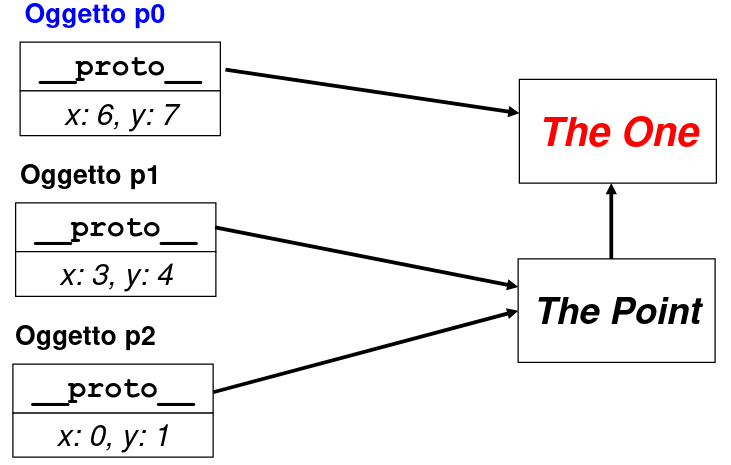
\includegraphics[width=0.4\textwidth]{/home/riccardoob/appunti/linguaggi/images/55.png}
\end{figure}

Esiste un prototipo predefinito per ogni categoria di oggetti: funzioni, array, numeri... ma tutti questi prototipo condividono a loro volta l'antenato comune, nasce così la tassonomia di prototipi che esprime l'ereditarietà.

\begin{figure}[H]
    \centering
    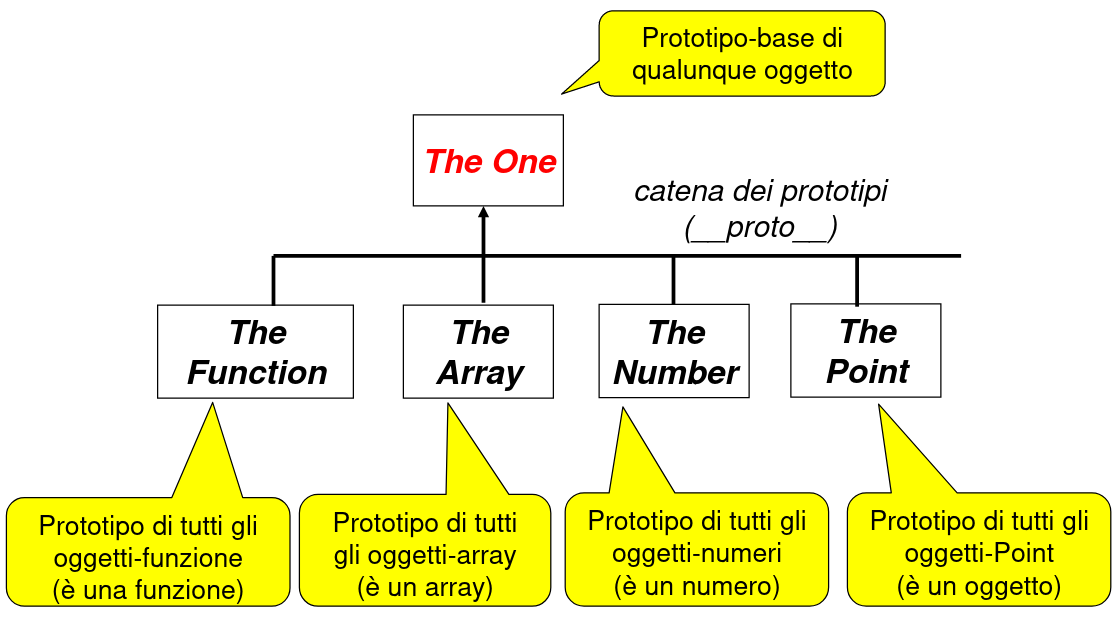
\includegraphics[width=0.6\textwidth]{/home/riccardoob/appunti/linguaggi/images/56.png}
\end{figure}

\subsection{Prototipi di costruzione}
Il prototipo di un oggetto dipende da \textit{chi lo costruisce}. La proprietà che definisce quale prototipo viene assegnato agli oggetti creati è \texttt{prototype} (riservata ai costruttori).

Spesso questa proprietà è chiamata \textbf{prototipo di costruzione}.

Tramite la proprietà \texttt{prototype} è possibile referenziare (indirettamente) gli oggetti predefiniti.

\subsection{Prototipi ed effetti a runtime}
Le relazioni fra oggetti espresse dalle catene di prototipi possono essere \textit{modificate a runtime}, in particolare è possibile
\begin{itemize}
    \item \textit{aggiungere/togliere} proprietà a un prototipo in uso
    \item \textit{sostituire} un oggetto-prototipo con un altro
\end{itemize}

\subsubsection{Type augmenting}
Per \textbf{type augmenting} si intende la possibilità di aggiungere proprietà a un prototipo esistente, causando un immediato impatto sugli oggetti già esistenti: la struttura del sistema cambia a runtime.

Per implementare questa funzionalità, si manipola la propritetà prototype del corrispondente costruttore.

\subsubsection{Creating e inheriting}
In alternativa, è possibile \textit{sostituire il prototipo di costruzione} con un altro, ciò non ha impatto sugli oggetti già esistenti ma avrà conseguenze sugli oggetti costruiti successivamente.

É il modo per definire un ereditarietà prototipale personalizzata, si reimposta la proprietà prototype agganciandola a un opportuno oggetto-prototipo.

\subsection{Ereditarietà prototype-based}
Per avere oggetti in relazione padre-figlio ("is a"), occorre \textit{impostare i prototipi di costruzione} in modo da \textit{riflettere la tassonomia desiderata}

\subsubsection{Esempio}
Esprimere che la categoria \texttt{Studente} \textit{eredita} dalla categoria \texttt{Persona}.

Occorre
\begin{itemize}
    \item definire il costruttore \texttt{Persona} con le relative proprietà
    \item definire il costruttore \texttt{Studente} con le relative proprietà
\end{itemize}

Per creare la gererchia, gli oggetti studente che saranno costruiti, dovranno avere come prototipo una persona.

\begin{minted}[bgcolor=lightgray,framesep=2mm,baselinestretch=1.2,fontsize=\footnotesize,escapeinside=||,mathescape=true]{js}
Persona = function(nome, annoNascita){
    this.nome = nome; this.anno = annoNascita;
    this.toString = function() {
        return this.nome + " è nata nel " + this.anno }
}

Studente = function(nome, annoNascita, matricola){
    this.nome = nome; this.anno = annoNascita;
    this.matricola = matricola;
    this.toString = function() {
        return this.nome + " è nata nel " + this.anno +
        " e la sua matricola è " + this.matricola }
}
\end{minted}

Si crea una specifica \texttt{Persona}, da usare come prototipo a tutti gli studenti.
\begin{minted}[bgcolor=lightgray,framesep=2mm,baselinestretch=1.2,fontsize=\footnotesize,escapeinside=||,mathescape=true]{js}
protoStudente = new Persona("zio", 1900);
\end{minted}

Si imposta il prototipo di \texttt{Studente} in modo che faccia riferimento a \texttt{protoStudente} e il suo costruttore a \texttt{Studente}.
\begin{minted}[bgcolor=lightgray,framesep=2mm,baselinestretch=1.2,fontsize=\footnotesize,escapeinside=||,mathescape=true]{js}
Studente.prototype = protoStudente;

Studente.prototype.constructor = Studente;
\end{minted}

\begin{figure}[H]
    \centering
    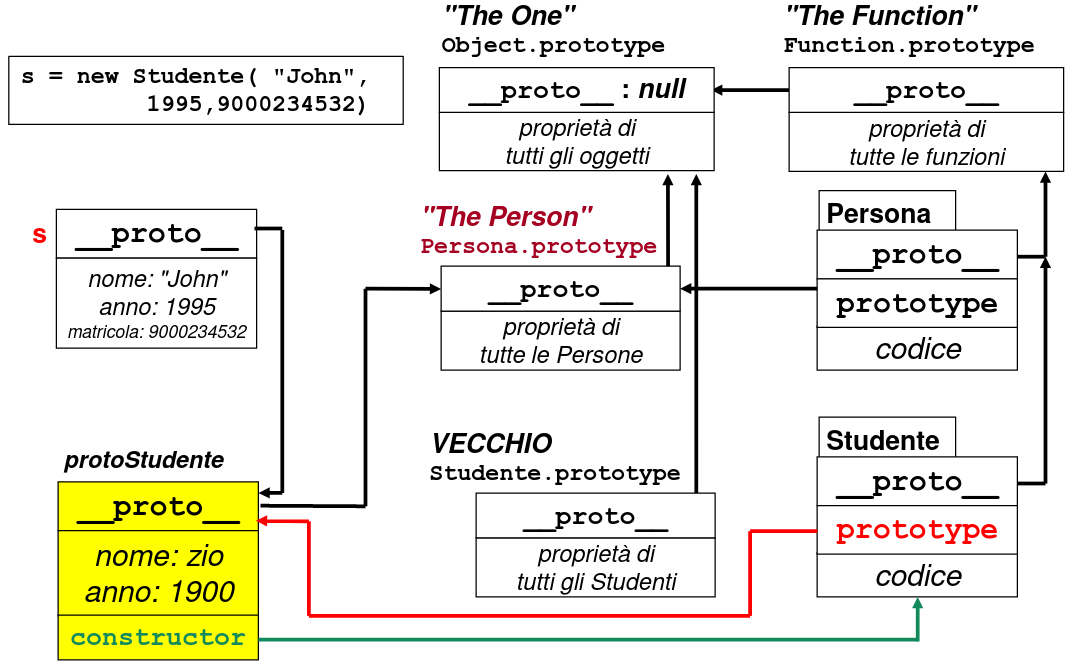
\includegraphics[width=0.6\textwidth]{/home/riccardoob/appunti/linguaggi/images/57.png}
\end{figure}

\subsubsection{Riferimenti alla classe base}
Non avendo l'idea di classe, non riesce a riferire la classe base (keyword \texttt{super}); tuttavia, tramite il metodo \texttt{call}, è possibile chiamare un oggetto-funzione.
\begin{minted}[bgcolor=lightgray,framesep=2mm,baselinestretch=1.2,fontsize=\footnotesize,escapeinside=||,mathescape=true]{js}
Studente = function(nome, annoNascita, matricola){
    Persona.call(this, nome, annoNascita);
    this.matricola = matricola;
    this.toString = function() {
        return Studente.prototype.toString.call(this) +
        " e la sua matricola è " + this.matricola }
}
\end{minted}

\subsection{Oggetto globale}
Javascript prevede un \textbf{ambiente globale} che ospita funzioni e variabili definite fuori da ogni altro scope.

É un opportuno oggetto, avente:
\begin{itemize}
    \item come metodi, tutte le funzioni predefinite
    \item più tutte le funzioni e le variabili globale definite dall'utente
\end{itemize}

Non è prestabilito, ma impostato dall'engine che esegue il codice (broswer $\rightarrow$ \texttt{window}, server $\rightarrow$ \texttt{response} ...).

\subsection{Simil classi}
Da ECMAScript 6, sono state introdotte le classi con la sintassi classica, che permette anche l'ereditarietà tramite keyword.

\section{Dove i due lati si incontrano}

\subsection{Costruire oggetti funzione}
Finore abbiamo utilizzato solo function literals, con il costruttore \texttt{Function} si possono costruire oggetti funzione dedicati a creare altri oggetti funzione: questo è un costrutto linguistico di \textbf{meta-livello}.

Come parametri prende soltanto stringhe, i primi N - 1 sono i nomi dei parametri, l'ultimo è il testo del corpo della funzione da creare.

\begin{minted}[bgcolor=lightgray,framesep=2mm,baselinestretch=1.2,fontsize=\footnotesize,escapeinside=||,mathescape=true]{js}
square = new Function("x", "return x*x")
\end{minted}



















